%\documentclass[t,handout]{beamer}
\documentclass{beamer}


\usepackage[utf8]{inputenc}
\usepackage[english]{babel}
%\usepackage[tight]{subfigure}
\usepackage{graphicx}
\usepackage{color}
\usepackage{url}
% \usepackage{listings}
%\usepackage[alf]{abntcite}


%\usetheme{Frankfurt} %LEGAL     !!!
% \usetheme{Madrid}     %LEGAL/L%IMPO/COM CAIXA     (sem barra de desenvolvimento)

% \usetheme{Antibes} %NAO
%\usetheme{Berlin} %PODE SER...     (BARRA DE DESENVOLVIMANTO)
% \usetheme{Berkeley}     %FEIO
% \usetheme{Boadilla} %TUDO BRANCO...
% \usetheme{Copenhagen}     %NAO
% \usetheme{Darmstadt} %LEGAL!     !!!
 \usetheme{Dresden}     %LEGAL/LIMPO/SEM CAIXA     (sem caixa fica ruim...)

% \usetheme{Goettingen}     %FEIO DEMAIS!
%\usetheme{Ilmenau} %LEGAL (forte candidato)
% \usetheme{JuanLesPins} %BACANA
% \usetheme{Luebeck}     %FEIO

% \usetheme{Malmoe}     %FEIO
% \usetheme{Warsaw} %NAO...
% \usetheme{Seattle}
% \usetheme{CambridgeUS}
% \usetheme{Singapore}

% \usecolortheme[RGB={130,35,150}]{structure}
% \usecolortheme[RGB={33,33,94}]{structure}
\usecolortheme[RGB={134,153,188}]{structure}
\setbeamertemplate{footline}[frame number]
\setbeamertemplate{navigation symbols}{}

%Hide subsections on teable of contents
%\hypersetup{bookmarksopen=true,bookmarksopenlevel=4}
%\setcounter{tocdepth}{2}



\author[]{\textbf{Leonardo Medeiros}, Hyggo Almeida, Leandro da Silva, Mirko Perkusich and Robert Fischer}

%\date{\today}
\date{23/06/2016}
\institute[]{Federal University Of Campina Grande - BRAZIL
}
\title{A Game-Based Approach to Monitor Parkinson's Disease: The bradykinesia symptom classification}
\logo{
\includegraphics[width=0.2\linewidth]{img/logo.png}}
\subtitle{\textbf{CBMS 2016}}

\begin{document}

\begin{frame}
  \titlepage
\end{frame}

% \section{Roteiro}
% \AtBeginSection[]
{\frame{
\frametitle{Summary}
%\tableofcontents
\tableofcontents
}
}






\section{Motivation}
\subsection{}
\begin{frame}{Health Monitoring Systems (HMS)}
  \begin{block}{}
Designed to support continuous treatment by moving healthcare services from the hospital to the patients' home. 
  \end{block} 
\end{frame}

\begin{frame}{The HMS's Major Challenge}
  \begin{block}{}
  \center
      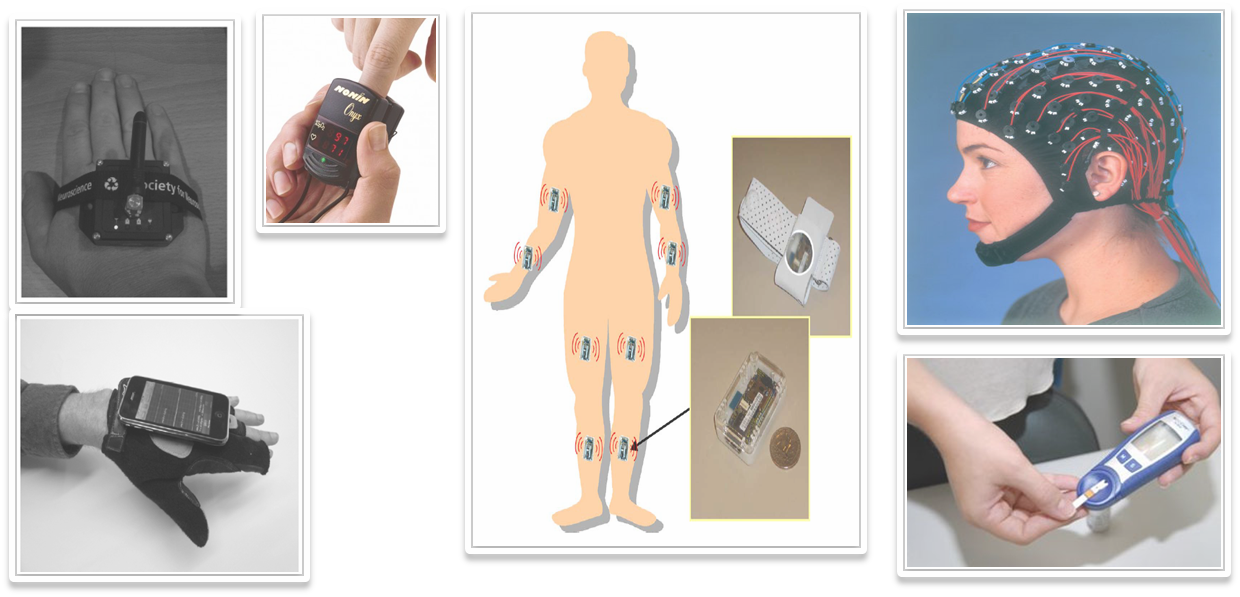
\includegraphics[height=1.8 in]{img/sismonsaude.png}
  \end{block}  
\end{frame}


\begin{frame}{Parkinson Disease (PD)}  
  \begin{block}{}
The symptoms associated with PD are caused by a \textbf{degeneration of dopaminergic neurons} in the substantia nigra. Common treatment focuses on \textbf{drugs that activate dopamine receptors}. However, the medication's effectiveness decreases over the years \textbf{requiring higher dosages}
  \end{block} 
\end{frame}

\begin{frame}{PD's Treatment and Disease Management} 
    \begin{block}{}
      \begin{itemize}
					\item Clinical trial evaluation: subjectively and sporadically;
					\item Motor fluctuations (\textit{on/off} phenomenon).
     \end{itemize}
  \end{block}
\end{frame}



\begin{frame}{Bradykinesia Symptom}
  \begin{block}{}
      \begin{itemize}
				\item Bradykinesia describes a slowness in the execution of movement. It is one of the four key symptoms of parkinsonism, which are bradykinesia, tremor, rigidity, and postural instability
				\item The tremmor is the most visible PD's motor symptom, but the bradykinesia is the most
	\end{itemize}
  \end{block}
\end{frame}
  


\section{Objectives}
\subsection{}
\begin{frame}{Main Objective}
		 \begin{block}{}
				A non-invasive HMS for Parkinson's Disease motor symptoms based on games to continuously provide data regarding patient, without reminding the disease's treatment
		 \end{block}
     \begin{block}{}
     \begin{center}		
		
      \end{center}
    \end{block}
\end{frame}

\begin{frame}{Main Requirements}
    \begin{block}{}
		    \begin{enumerate}[<+->]
            \item A contactless measurement of patient motor symptoms inside the game environment;
						\item Use of a popular consumer electronic device as input to have a non-invasive, cost-effective solution for home use.
        \end{enumerate}
    \end{block}
\end{frame}

%
\begin{frame}{Who will use the Game-Based Health Monitor Approach}
    \begin{block}{}
        \begin{itemize}[<+->]
            \item A person with age above 55 years old;
            \item A person with Parkinson's disease;
            \item Neurologist and physiotherapist responsible for patient's treatment.
        \end{itemize}
    \end{block}
\end{frame}


\begin{frame}{Use Scenario}
   \begin{block}{}
      \begin{itemize}[<+->]
       \item A PD' patient play the \textbf{HGM Client} in home and seamlessly provide the motor data;
       \item So, the motor signs are sent to \textbf{HGM Server};
       \item The HGM Server process the user's data and identify the occurrence of the PD's disease bradykinesia symptom;
       \item Then, the \textbf{neurologist visualize} the \textbf{user's health information} to assess the patient's \textbf{level of motor deficiency}.
      \end{itemize}
  \end{block}
\end{frame}

%\begin{frame}{System Overview}
		 %\begin{block}{}
			%\begin{center}
				%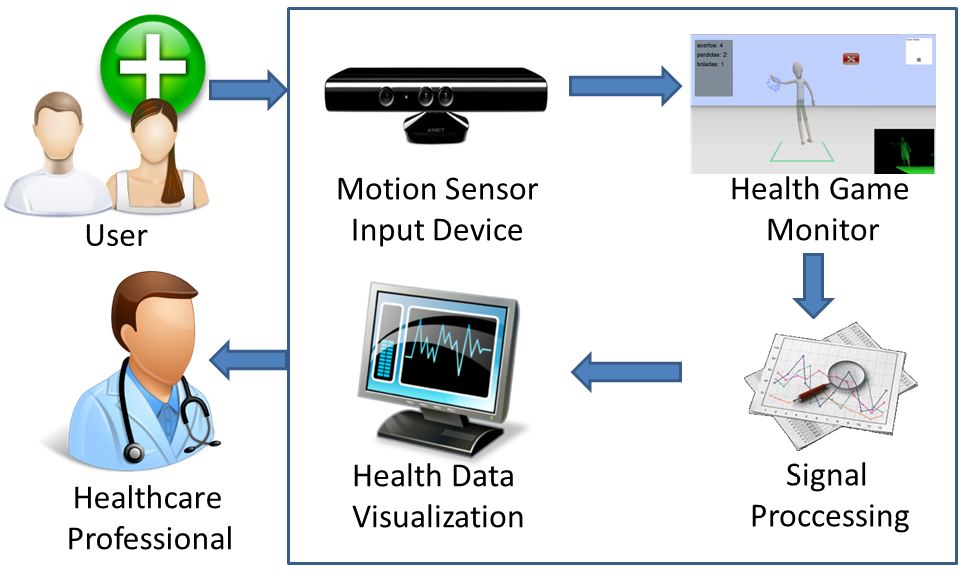
\includegraphics[height=2.2 in]{img/systemoverview3.png}
			%\end{center}
		 %\end{block}
%\end{frame}


\begin{frame}{What was developed?}
    \begin{block}{}
        \begin{itemize}[<+->]
            \item  A semi-structured interview with healthcare professionals associated to scientific references to identify the system requirements;
            \item The development of the Health Game Monitor (HGM) Client (Catch the Spheres' game);
            \item The development of the HGM Server, responsible for processing the data and making the results available to the health professional;
						\item Experimental studies with target users.
        \end{itemize}
    \end{block}
\end{frame}

\section{System Requirements}
\subsection{}
\begin{frame}{Qualitative Research Analysis} 
    \begin{block}{}					
		The respondents suggested focusing on the bradykinesia motor symptom due to its debilitating progress. Thus, treatment benefits could be correlated with the \textbf{increase of amplitude and angular velocities of an arm's adduction and abduction movements}.
    \end{block}
\end{frame} 




\begin{frame}{Some Elicited Requirements}
	\begin{block}{}
		\begin{itemize}[<+->]
			\item	Easy and safe to use equipment
      \item Incite the player to perform specific movements that are required for the measurement 
      \item Game with clear and entertaining goal and adapted to the user's skills
			\item Provide a informative visual way to the healthcare professional
		\end{itemize}
	\end{block}
\end{frame}




\section{System Development}
\subsection{}
\begin{frame}{System Architecture}
		 \begin{block}{}
			\begin{center}
				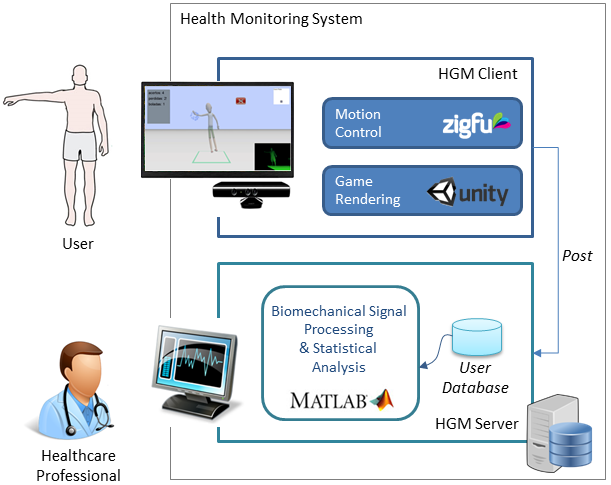
\includegraphics[height=2.2 in]{img/systemarchitecture3.png}
			\end{center}
		 \end{block}
\end{frame}

\begin{frame}{Biomechanical signal processing}
	\begin{block}{}
		\begin{center}
				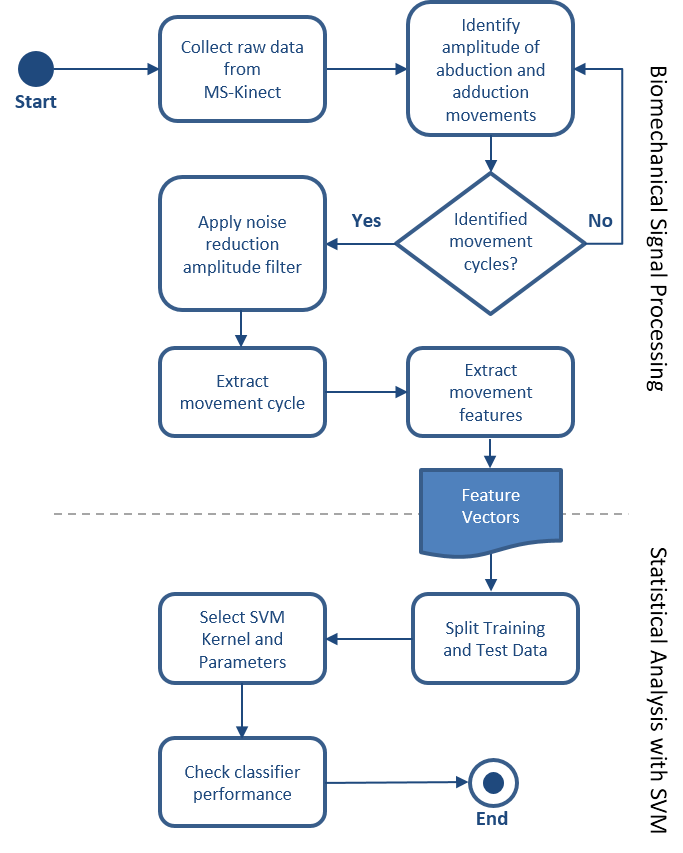
\includegraphics[height=2.2 in]{img/biomecprocessor2.png}
		\end{center}
	\end{block}
\end{frame}


%\begin{frame}{The Biomechanical Analysis of Human Movement}
  %\begin{block}{}
   %The diagnosis and treatment process for PD uses the biomechanical analysis of human movement, where the patients are asked to lift their arms, one after the other, at the highest amplitude and velocity they are able to, in order to check the bradykinesia progress. 
  %\end{block}
%\end{frame}

\begin{frame}{Ms-Kinect Joints Acquisition}
  \begin{block}{}
      \center 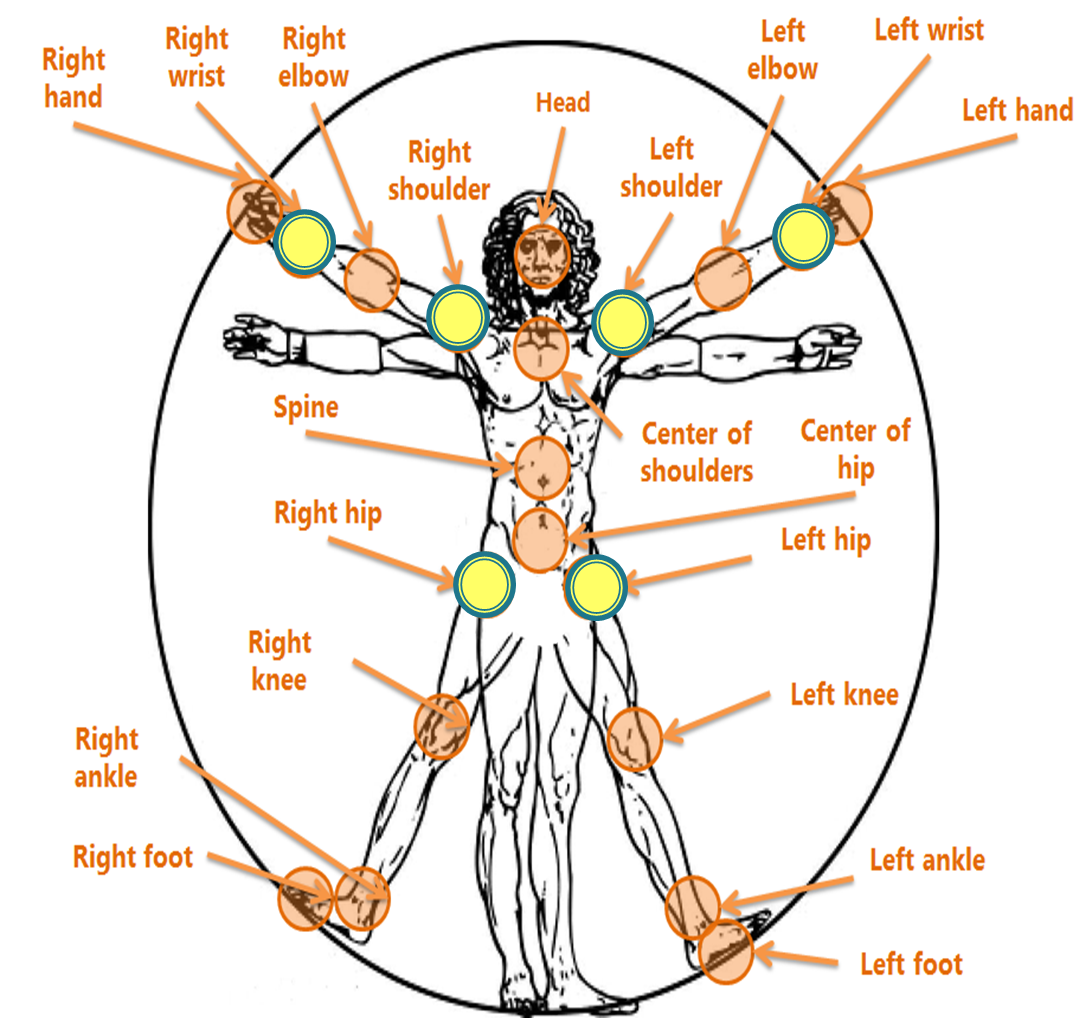
\includegraphics[height=2.5 in]{img/articulacoes-sel.png}
			%\caption{Modificações no Jogo ao Longo das Fases de Desenvolvimento~\cite{fullerton2008game}}
  \end{block}
	
	\begin{block}{}
	Adduction and Abduction involves: \textbf{wrist, shoulder, and hip} joints.
	\end{block}	
\end{frame}



\begin{frame}{Angle over time with the peak and valley detection technique}
  \begin{block}{}
      \center 
      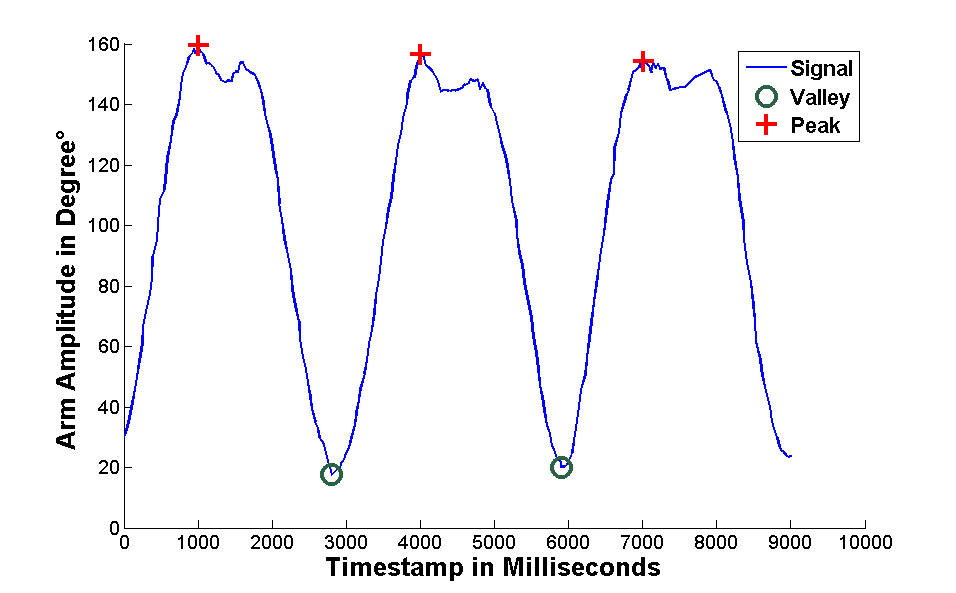
\includegraphics[height=1.6 in]{img/signalamplitudepeakvaley-2.png}
  \end{block}
	
	\begin{block}{}
	The cycle movement and transform the MS-Kinect data into angles. Thus, we calculate the \textbf{angular motion} of the adduction and abduction movements.
	\end{block}
\end{frame}

\begin{frame}{Some Elicited Requirements}
	\begin{block}{}
		\begin{itemize}[<+->]
			\item	Easy and safe to use equipment
      \item Incite the player to perform specific movements that are required for the measurement 
      \item Game with clear and entertaining goal and adapted to the user's skills
			\item Provide a informative visual way to the healthcare professional
		\end{itemize}
	\end{block}
\end{frame}

\begin{frame}{Developed Health Game Monitor: Catch the Spheres}
	\begin{center}
      \center 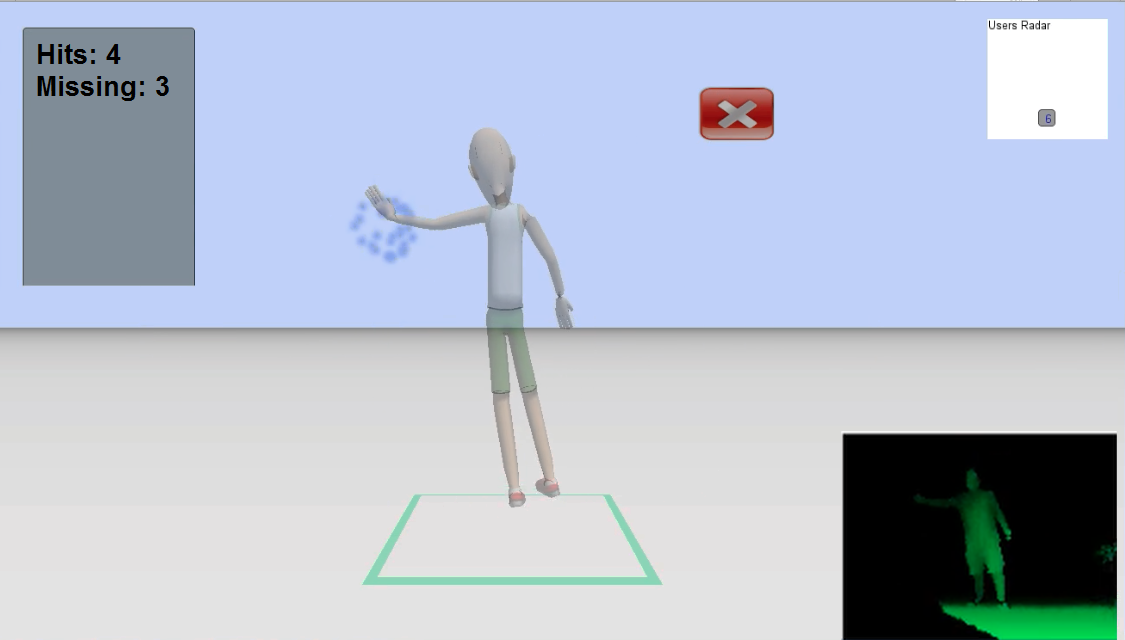
\includegraphics[height=2.2 in]{img/catch_colour.png}
	\end{center}
\end{frame}

\section{Experiments}
\subsection{}
\begin{frame}{Case Control Study}
	\begin{block}{}
	A total number of 30 subjects participated where 15 subjects for each group.
		\begin{itemize}
			\item PD' Group: 10 men and 5 women, between 51 and 65 years (mean: 58);
			\item Control Group: 11 men and 4 women, between 50 and 65 years (mean: 57).
		\end{itemize}
	\end{block}
\end{frame}

\begin{frame}{Procedure for Data Collection}
	\begin{block}{}
	\begin{compactenum}
	\item The subject stands at distance of 2 meters from the motion sensor at a place marked for that purpose on the ground;
	\item The subject faces a projection of the game on a wall, centered over the motion sensor;
	\item The subject plays the game \textit{Catch the Spheres} for 5 minutes;
	\item The subjects end the game by reaching the virtual exit button.
\end{compactenum} 
	\end{block}
\end{frame}


\begin{frame}{Data Classifier: SVM}
\begin{block}{}
	In this work, we used Support Vector Machine (SVM) as the supervised learning method. SVM seeks to find a margin that separates all positive and negative example.
		
	We choice this algorithm because he has \textbf{a good generalization to discriminate between two classes}.
\end{block}
\end{frame}



\begin{frame}{SVM Classifier Performance}
   \begin{block}{}
   
   \begin{columns}[c]
     \begin{column}{0.5\linewidth}
				\begin{table}[!htbp]
					\label{table:resultadomatrizconfusaosvm}
					\centering
					\begin{tabular}{l|c|c|}
					\cline{2-3}
					\multicolumn{1}{c}{}                         & \multicolumn{2}{|c|}{\textit{\textbf{Predictive Class}}} \\ \cline{2-3} 
																											 & \textbf{Parkinson}      & \textbf{Control}         \\ \hline
					\multicolumn{1}{|l|}{\textbf{Parkinson}} & 12       & 3           \\ \hline
					\multicolumn{1}{|l|}{\textbf{Control}}     & 1           & 14     \\ \hline
					\end{tabular}
			\end{table}

     \end{column}

     \begin{column}{0.55\linewidth}
						\begin{table}[htbp!]
						\begin{tabular}{|l|r|}
						\hline
						\multicolumn{2}{|l|}{\textbf{Classifier Metrics}} \\ \hline
						\textbf{TpRate}                    & 80.00$\%$\                 \\ \hline
						\textbf{FpRate}                    & 6.67$\%$\                \\ \hline
						\textbf{Accuracy}                  & 86.67$\%$\                \\ \hline
						\textbf{F-score}                   & 85.71$\%$\                \\ \hline
						\textbf{Precision}                  & 92.31$\%$\                \\ \hline
						\end{tabular}
						\end{table}
    \end{column}
\end{columns}
\end{block}
\end{frame}

%\subsection{User Acceptance}
\begin{frame}{Goal Question Metric (GQM) for User Acceptance}
	\begin{block}{}
	Based on the GQM paradigm, we defined two goals:
		\begin{description}
			\item [G1]: Analyze our HMS PD approach for the purpose of evaluating with respect to usability from the view point of the patients in the context of the game \emph{Catch the Spheres}
			\item [G2]: Analyze our HMS PD approach for the purpose of evaluating with respect to fit to daily routine from the view point of the patients in the context of the game \emph{Catch the Spheres}
		\end{description}
	\end{block}
\end{frame}


\begin{frame}{GQM Results}
	\begin{block}{}
	The measurements were collected we obtained the following result indicating:
		\begin{itemize}
			\item 90\% of the users felt motivated with the game;
			\item 80\% would add this game-based monitoring approach into their daily routine; 
			\item 75\% considered it safe for elderly users.
		\end{itemize}
	\end{block}
\end{frame}

\section{Conclusion}
\subsection{}
\begin{frame}{Conclusion}
	\begin{block}{}
	In this work we presented a game-based approach to monitor with a symptom classification \textit{Precision} of 92.31\%. Moreover, 90,00\% of the patients considered our approach non-invasive and easy to integrate into their routine. 
	\end{block}
\end{frame}

%\subsection{Dúvidas}
\begin{frame}
  \begin{center}
  Questions ?
  \end{center}
\end{frame}

\bibliographystyle{IEEEtran}
\bibliography{sigproc2,IEEEFormat}

\end{document}
	